\paragraph{Historical attack chain.}

\begin{enumerate}
    \item \textbf{Windows infection:} Stuxnet entered internal networks via USB and spread using Windows zero-days, reporting to C\&C servers~\cite{falliere2010stuxnet,stuxnet_work_details}.
    \item \textbf{Step~7 hooking (*):} On each infected workstation it hooked \texttt{s7otbxdx.dll} to intercept and modify traffic between Step~7 and the PLC---a software-layer man-in-the-middle attack (Figures~\ref{fig:stuxnet_mitm_sim-image-9} and~\ref{fig:stuxnet_mitm_sim-image-10}).
    \item \textbf{Centrifuge control interference:} Stuxnet modified PLC logic to raise centrifuge speed above safe limits. Malicious code was injected via Step~7, executed on the PLC, forwarded to the variable frequency drive (VFD), and physically damaged the centrifuge while falsified values were sent to WinCC.
\end{enumerate}

\begin{figure}[htbp]
    \centering
    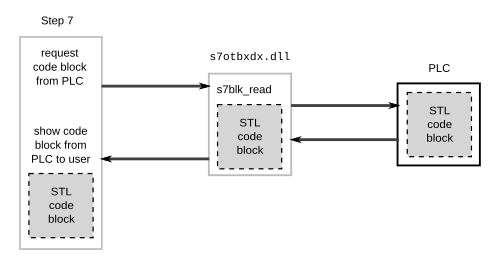
\includegraphics[width=0.85\textwidth]{../attacks/stuxnet_mitm_sim/image-9.png}
    \caption{Normal Step~7--PLC communication}
    \label{fig:stuxnet_mitm_sim-image-9}
\end{figure}

\begin{figure}[htbp]
    \centering
    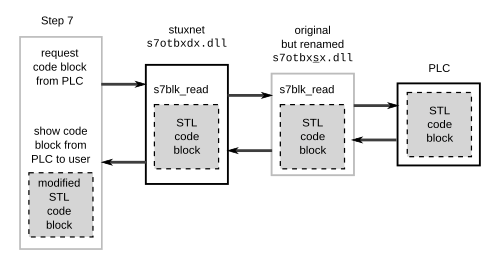
\includegraphics[width=0.85\textwidth]{../attacks/stuxnet_mitm_sim/image-10.png}
    \caption{Stuxnet MITM on Step~7--PLC link}
    \label{fig:stuxnet_mitm_sim-image-10}
\end{figure}



Stuxnet activated only when the target PLC and drive matched narrow criteria: Siemens S7-300, Vacon or Fararo Paya drives, and operating frequency between 807~Hz and 1210~Hz---typical of gas centrifuges rather than ordinary industrial equipment. When matched, it stepped output frequency through levels such as 1410~Hz, 2~Hz, and 1064~Hz to damage the process while concealing the effect on monitoring data.

\textit{In this thesis, the same operational outcome is reproduced at the S7comm network layer (Figure~\ref{fig:lab-topology}) rather than via DLL hooking as in the historical campaign.}

(*) \textit{TIA Portal bundles STEP~7, WinCC, PLCSIM, and drive configuration tools for Siemens S7 PLC families.}

\paragraph{Attack simulation.}

The lab reproduces the same \emph{operational} outcome as the historical campaign---change what the PLC executes while keeping the operator display unchanged---but implements it on the wire rather than inside Step~7 libraries. The scenario therefore has three layers that must be prepared before the attack runs: a PLC program that exposes the process variables of interest, an HMI that polls those variables over S7comm, and an attacker host that can both write the PLC and sit on the HMI--PLC path. The subsections below describe each layer; the attacker stage then combines an unauthorized write, ARP redirection, and in-flight editing of Read~Var responses.

\subsubsection{PLC setup}

The scenario control program is imported into OpenPLC Editor from the project bundle supplied with the lab. Because OpenPLC allows only one data type per datablock, inputs and outputs are split across DB1 and DB2 (Figure~\ref{fig:stuxnet_mitm_sim-image-1}). Structured Text logic drives simulated motor speed oscillating around setpoint \texttt{iSetpoint = 1200} (Figure~\ref{fig:stuxnet_mitm_sim-image-2}).

\begin{figure}[htbp]
    \centering
    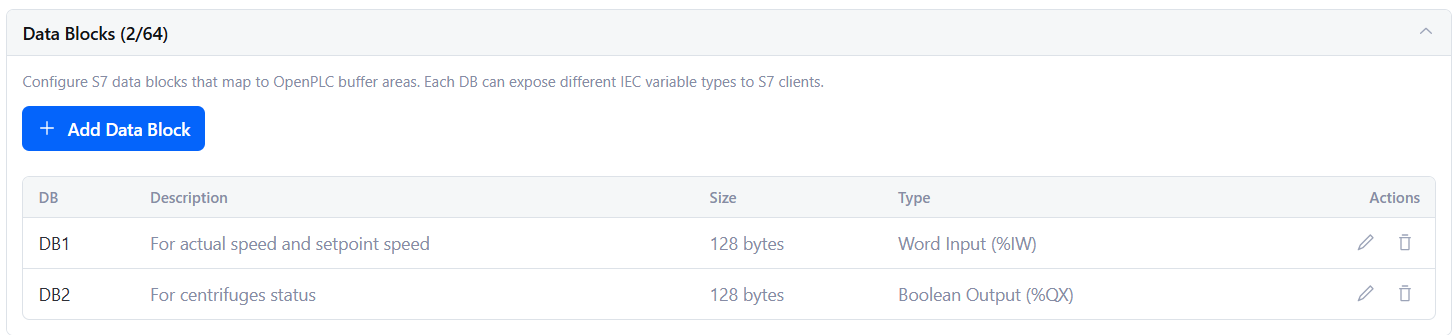
\includegraphics[width=0.85\textwidth]{../attacks/stuxnet_mitm_sim/image-1.png}
    \caption{OpenPLC datablocks DB1 and DB2}
    \label{fig:stuxnet_mitm_sim-image-1}
\end{figure}

\begin{figure}[htbp]
    \centering
    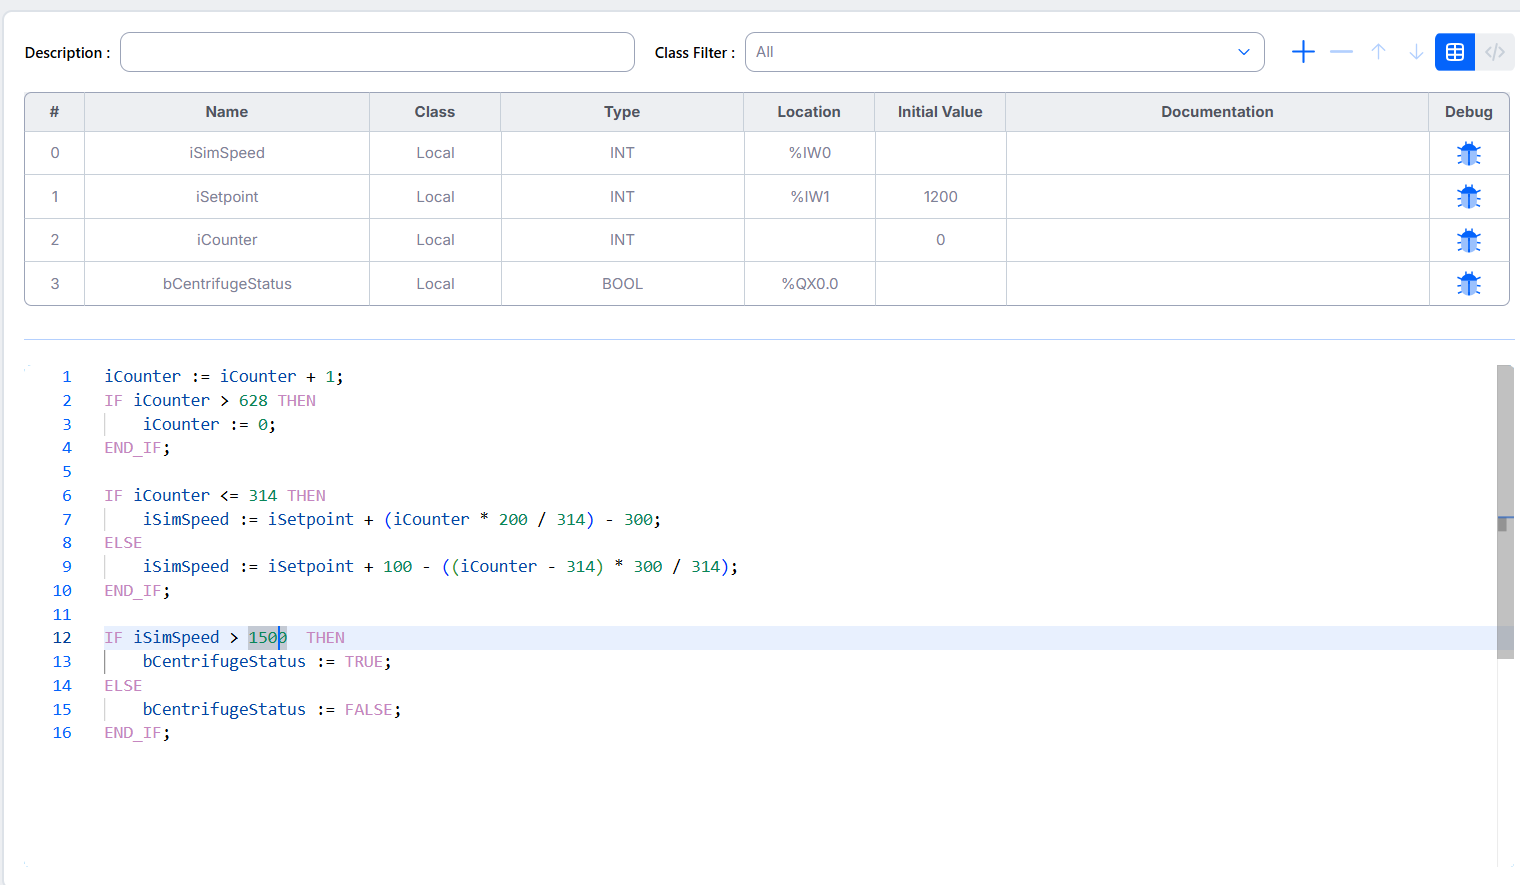
\includegraphics[width=0.85\textwidth]{../attacks/stuxnet_mitm_sim/image-2.png}
    \caption{Structured Text tags and logic}
    \label{fig:stuxnet_mitm_sim-image-2}
\end{figure}

The tags used later in traffic analysis are \texttt{iSimSpeed} and \texttt{iSetpoint} in DB1 (16-bit words), \texttt{iCounter} for the oscillation pattern, and \texttt{bCentrifugeStatus} in DB2 (0 = normal, 1 = overspeed above 1500~Hz). Once compiled and loaded, the runtime serves these variables on TCP/102 like a Siemens CPU.

\subsubsection{HMI setup}

The supervisory project is imported into FUXA and bound to the same PLC tags (Figure~\ref{fig:stuxnet_mitm_sim-image-8}). Under normal operation the HMI shows speed near 1200 in green, consistent with the OpenPLC debugger (Figure~\ref{fig:stuxnet_mitm_sim-image-17}). The program must remain loaded in the runtime before the HMI connects; otherwise polling will fail or show stale values.

\begin{figure}[htbp]
    \centering
    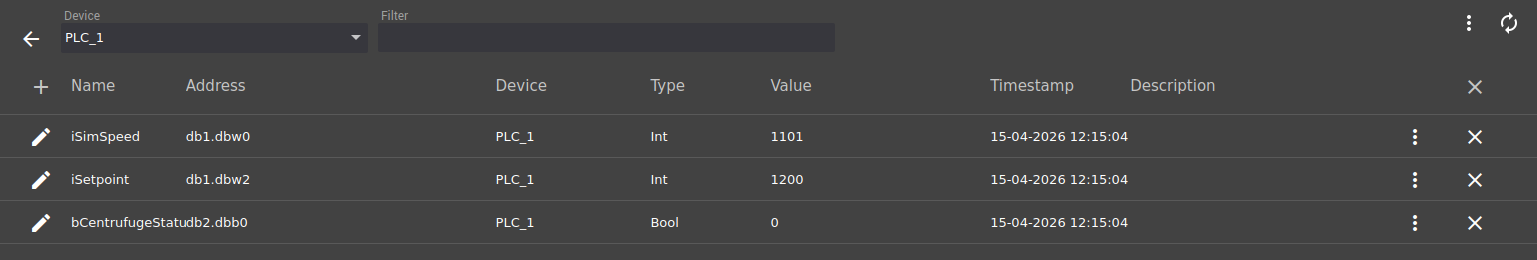
\includegraphics[width=0.85\textwidth]{../attacks/stuxnet_mitm_sim/image-8.png}
    \caption{FUXA project import and tags}
    \label{fig:stuxnet_mitm_sim-image-8}
\end{figure}

\begin{figure}[htbp]
    \centering
    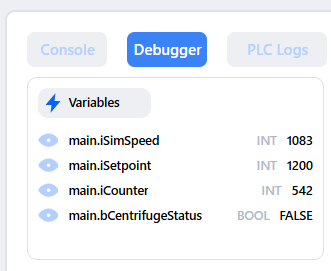
\includegraphics[width=0.85\textwidth]{../attacks/stuxnet_mitm_sim/image-17.png}
    \caption{OpenPLC Editor debugger view}
    \label{fig:stuxnet_mitm_sim-image-17}
\end{figure}

During steady-state polling, HMI--PLC traffic repeats two Read~Var request--response pairs: a 4-byte read of \texttt{iSimSpeed} and \texttt{iSetpoint} in DB1 (Figures~\ref{fig:stuxnet_mitm_sim-image-4} and~\ref{fig:stuxnet_mitm_sim-image-5}), and a 1-byte read of \texttt{bCentrifugeStatus} in DB2 (Figures~\ref{fig:stuxnet_mitm_sim-image-6} and~\ref{fig:stuxnet_mitm_sim-image-7}). Multi-byte values appear little-endian in the captures (\texttt{iSimSpeed} = \texttt{0x042d} $\rightarrow$ 1069; \texttt{iSetpoint} = \texttt{0x04b0} $\rightarrow$ 1200). These captures establish the baseline against which the MITM stage is compared.

\begin{figure}[htbp]
    \centering
    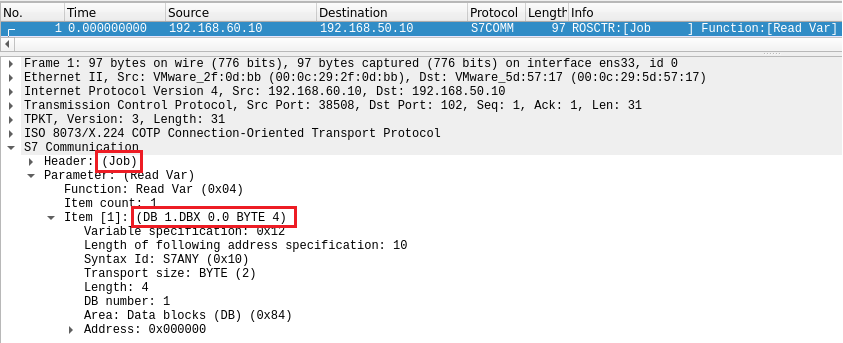
\includegraphics[width=0.85\textwidth]{../attacks/stuxnet_mitm_sim/image-4.png}
    \caption{Read Var request: DB1 variables}
    \label{fig:stuxnet_mitm_sim-image-4}
\end{figure}

\begin{figure}[htbp]
    \centering
    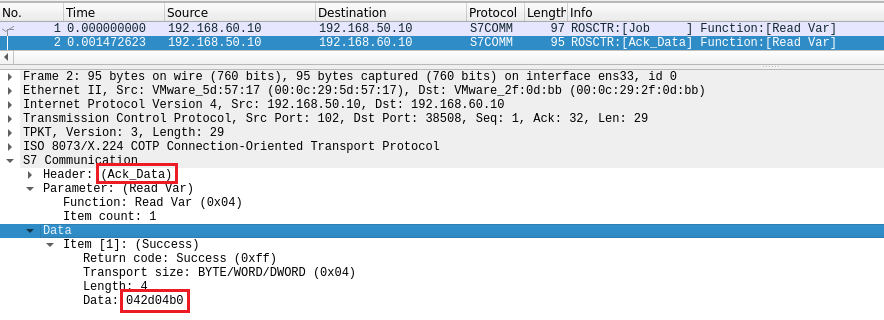
\includegraphics[width=0.85\textwidth]{../attacks/stuxnet_mitm_sim/image-5.png}
    \caption{Read Var response: DB1 variables}
    \label{fig:stuxnet_mitm_sim-image-5}
\end{figure}

\begin{figure}[htbp]
    \centering
    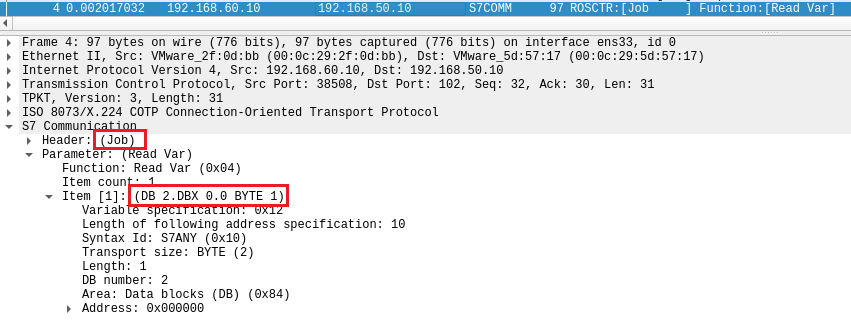
\includegraphics[width=0.85\textwidth]{../attacks/stuxnet_mitm_sim/image-6.png}
    \caption{Read Var request: status tag}
    \label{fig:stuxnet_mitm_sim-image-6}
\end{figure}

\begin{figure}[htbp]
    \centering
    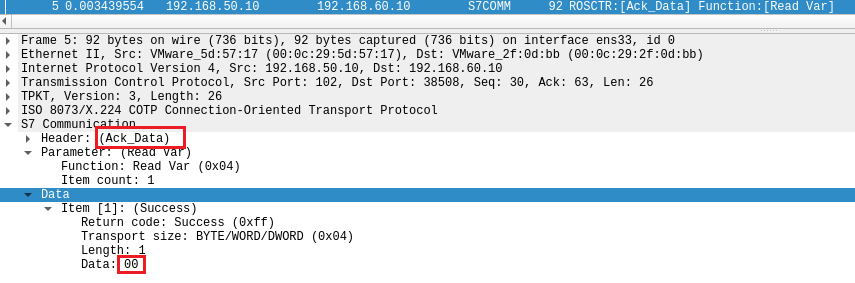
\includegraphics[width=0.85\textwidth]{../attacks/stuxnet_mitm_sim/image-7.png}
    \caption{Read Var response: normal status}
    \label{fig:stuxnet_mitm_sim-image-7}
\end{figure}

\subsubsection{Attacker stage}

With PLC and HMI running normally, the attacker host executes three coordinated actions. Step~1 changes the physical setpoint on the PLC; step~2 forces HMI-bound traffic through the attacker; step~3 restores the old setpoint only in responses destined for the HMI. Steps~2 and~3 must be active before step~1 matters to the operator display, but all three run concurrently in the lab script.

\begin{enumerate}
    \item \textbf{Unauthorized write.} From the attacker workstation, a Snap7 or Python S7comm client opens a session to the PLC and issues \texttt{Write Var} on \texttt{DB1.DBW2} (\texttt{iSetpoint}), changing the value from 1200 to 2000. No credential or session binding is required on classic S7comm~\cite{inprotech_s7comm_security}; possession of network reachability and memory addressing is sufficient.

    \item \textbf{ARP spoofing.} Bettercap poisons the ARP cache between the supervisory subnet gateway (\texttt{192.168.60.1}) and the HMI (\texttt{192.168.60.10}) in full-duplex mode so both HMI$\rightarrow$PLC and PLC$\rightarrow$HMI legs traverse the attacker before reaching their true destination.

    \item \textbf{Response forgery.} Packets redirected to the attacker are handed to a Linux NFQUEUE handler. The handler parses each S7comm \texttt{Ack\_Data} Read~Var response and rewrites \texttt{iSetpoint} from 2000 back to 1200 before reinjecting the frame toward the HMI.
\end{enumerate}

After the write alone (without steps~2--3), debugger and HMI both reflect the new setpoint. The packet dump below contrasts nominal operation with the post-write state:

\begin{packetdump}
    Current Speed  | Setpoint Speed    | Centrifuge Status
    --------------------------------------------------
    b'\x03\xc1'    |    b'\x04\xb0'    |    b'\x00'
    b'\x07\xe4'    |    b'\x07\xd0'    |    b'\x01'
\end{packetdump}

Here \texttt{iSetpoint} moves from \texttt{0x04b0} to \texttt{0x07d0} and \texttt{bCentrifugeStatus} becomes~1 because simulated speed exceeds 1500~Hz. Without MITM, the HMI trend turns red around 2000 (Figure~\ref{fig:stuxnet_mitm_sim-image-14}) and Wireshark shows the updated setpoint in PLC$\rightarrow$HMI traffic (Figure~\ref{fig:stuxnet_mitm_sim-image-15}).

\begin{figure}[htbp]
    \centering
    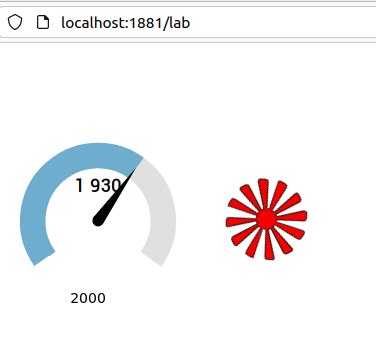
\includegraphics[width=0.55\textwidth]{../attacks/stuxnet_mitm_sim/image-14.png}
    \caption{HMI view without MITM}
    \label{fig:stuxnet_mitm_sim-image-14}
\end{figure}

\begin{figure}[htbp]
    \centering
    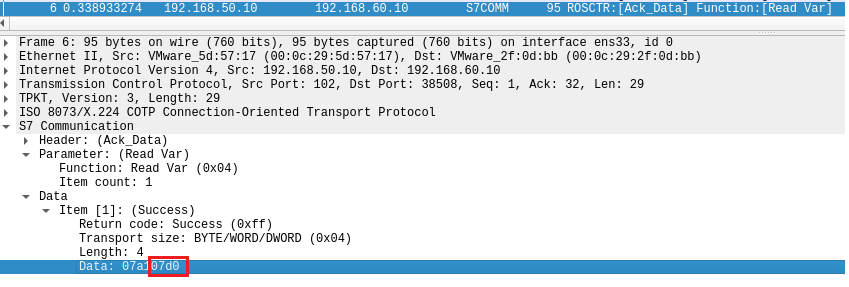
\includegraphics[width=0.85\textwidth]{../attacks/stuxnet_mitm_sim/image-15.png}
    \caption{Wireshark: updated setpoint in traffic}
    \label{fig:stuxnet_mitm_sim-image-15}
\end{figure}

When ARP spoofing and response forgery are enabled together with the write, Wireshark on the HMI segment shows S7comm frames interleaved with spoofing traffic (Figure~\ref{fig:stuxnet_mitm_sim-image-13}). The operator screen still displays setpoint~1200 and nominal colouring (Figure~\ref{fig:stuxnet_mitm_sim-image-18}), while forwarded \texttt{Ack\_Data} payloads carry the forged word \texttt{0x04b0} (Figure~\ref{fig:stuxnet_mitm_sim-image-28}). The overspeed status byte may still read~1 in a separate response (Figure~\ref{fig:stuxnet_mitm_sim-image-29}), so concealment is partial rather than complete. The OpenPLC debugger, which is not on the spoofed path, continues to show execution near the written value of 2000 (Figure~\ref{fig:stuxnet_mitm_sim-image-3}).

\begin{packetdump}
    set arp.spoof.targets 192.168.60.1, 192.168.60.10
    set arp.spoof.internal true
    set arp.spoof.fullduplex true
    arp.spoof on
\end{packetdump}

\begin{figure}[htbp]
    \centering
    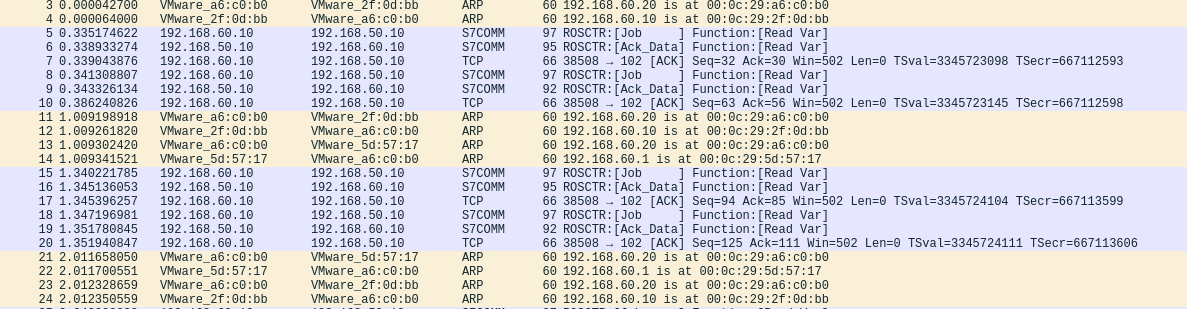
\includegraphics[width=0.85\textwidth]{../attacks/stuxnet_mitm_sim/image-13.png}
    \caption{S7comm and ARP spoofing packets interleaved}
    \label{fig:stuxnet_mitm_sim-image-13}
\end{figure}

\begin{figure}[htbp]
    \centering
    
\includegraphics[width=0.55\textwidth]{../attacks/stuxnet_mitm_sim/image-18.png}
    \caption{HMI view with MITM: nominal setpoint display}
    \label{fig:stuxnet_mitm_sim-image-18}
\end{figure}

\begin{figure}[htbp]
    \centering
    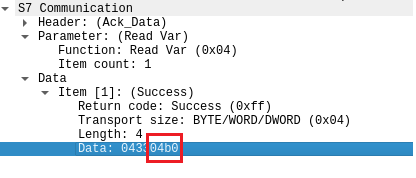
\includegraphics[width=0.85\textwidth]{../attacks/stuxnet_mitm_sim/image-28.png}
    \caption{Wireshark: forged setpoint field}
    \label{fig:stuxnet_mitm_sim-image-28}
\end{figure}

\begin{figure}[htbp]
    \centering
    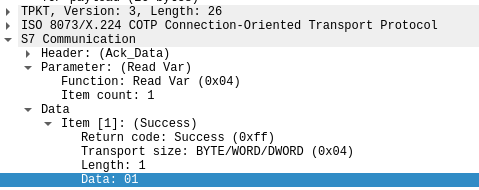
\includegraphics[width=0.85\textwidth]{../attacks/stuxnet_mitm_sim/image-29.png}
    \caption{Wireshark: overspeed status byte}
    \label{fig:stuxnet_mitm_sim-image-29}
\end{figure}

\begin{figure}[htbp]
    \centering
    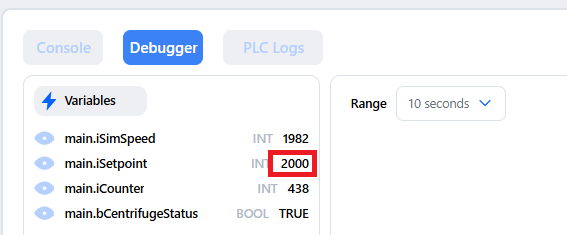
\includegraphics[width=0.85\textwidth]{../attacks/stuxnet_mitm_sim/image-3.png}
    \caption{OpenPLC debugger at actual speed}
    \label{fig:stuxnet_mitm_sim-image-3}
\end{figure}

In summary, the operator sees nominal setpoint 1200 on FUXA while the PLC debugger confirms logic running against the attacker-written value near 2000---the same deception pattern Stuxnet achieved through Step~7 hooks, reproduced here at the network layer.

\subsubsection{Attack analysis}

Network-layer forgery differs from DLL hooking because the attacker must parse and rewrite complete Ethernet frames at line rate. Bettercap alone is insufficient: its script interface cannot host a full S7comm parser, so the lab combines ARP redirection with the Linux NFQUEUE framework. Before queuing, the attacker enables IP forwarding, relaxes reverse-path filtering, adds a route to the PLC subnet, and installs \texttt{iptables} rules that copy TCP/102 flows into NFQUEUE. A userspace handler then receives each copied packet, validates the TPKT/COTP/S7 envelope, and either forwards unchanged or edits selected fields.

To know \emph{which} bytes to edit, the handler must understand Read~Var layout. An S7 PDU on TCP/102 stacks TPKT, COTP, an S7 header, and Param/Data sections (Figure~\ref{fig:iemensS7protocolstackpng}). Figures~\ref{fig:stuxnet_mitm_sim-image-19} and~\ref{fig:stuxnet_mitm_sim-image-20} show the framing layers; Figures~\ref{fig:stuxnetmitmsimimage25png} and~\ref{fig:stuxnetmitmsimimage26png} show representative Job and Ack\_Data Read~Var exchanges. The S7 header begins with protocol id~\texttt{0x32}; byte~8 (\texttt{ROSCTR}) distinguishes Job (\texttt{0x01}), Ack (\texttt{0x02}), and Ack\_Data (\texttt{0x03}).

\begin{figure}[htbp]
    \centering
    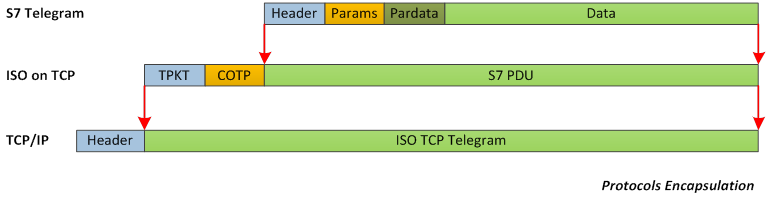
\includegraphics[width=0.9\textwidth]{../attacks/stuxnet_mitm_sim/Siemens_S7_protocol_stack.png}
    \caption{Siemens S7 protocol stack}
    \label{fig:iemensS7protocolstackpng}
\end{figure}

\begin{figure}[htbp]
    \centering
    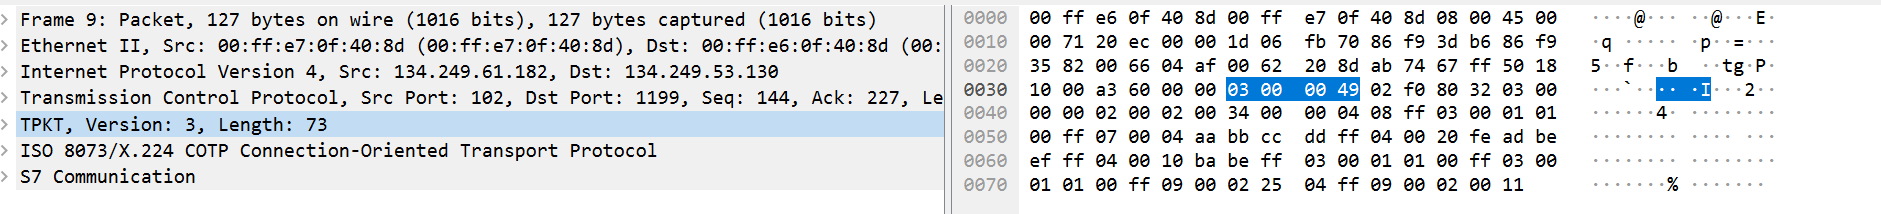
\includegraphics[width=0.9\textwidth]{../attacks/stuxnet_mitm_sim/image-19.png}
    \caption{TPKT header}
    \label{fig:stuxnet_mitm_sim-image-19}
\end{figure}

\begin{figure}[htbp]
    \centering
    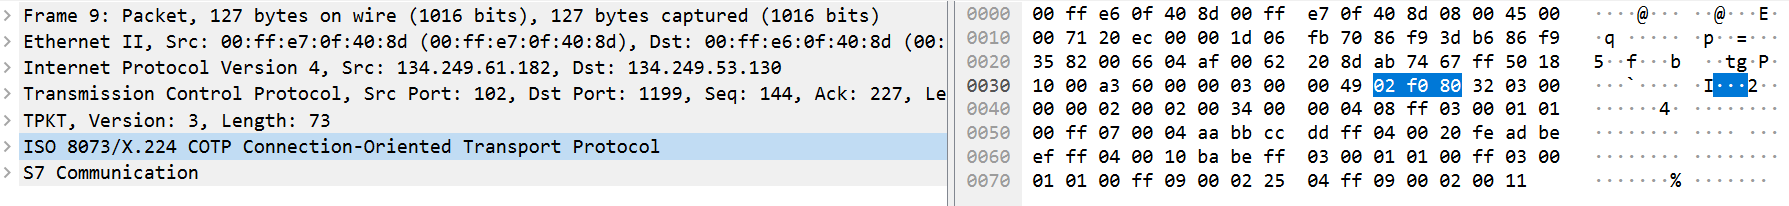
\includegraphics[width=0.9\textwidth]{../attacks/stuxnet_mitm_sim/image-20.png}
    \caption{COTP header}
    \label{fig:stuxnet_mitm_sim-image-20}
\end{figure}

\begin{figure}[htbp]
    \centering
    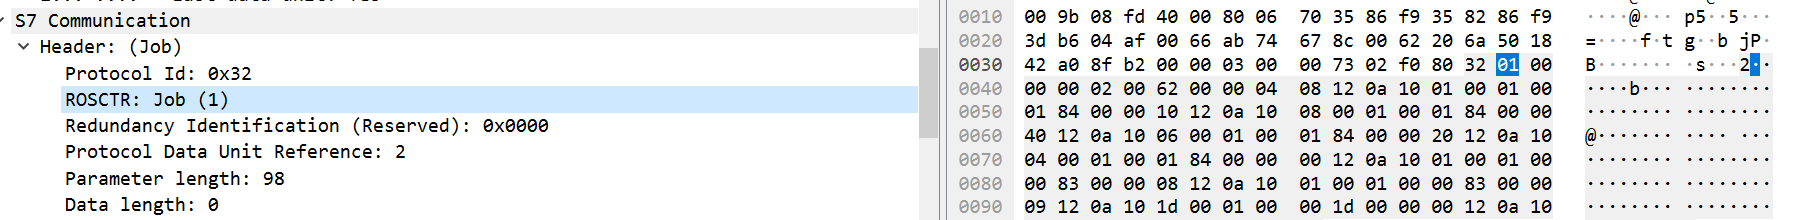
\includegraphics[width=0.9\textwidth]{../attacks/stuxnet_mitm_sim/image-25.png}
    \caption{Read Var request (Job PDU)}
    \label{fig:stuxnetmitmsimimage25png}
\end{figure}

\begin{figure}[htbp]
    \centering
    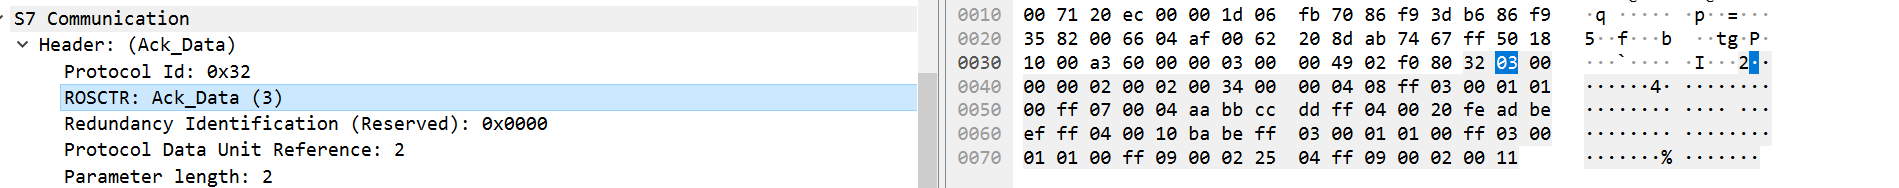
\includegraphics[width=0.9\textwidth]{../attacks/stuxnet_mitm_sim/image-26.png}
    \caption{Read Var response (Ack\_Data PDU)}
    \label{fig:stuxnetmitmsimimage26png}
\end{figure}

In the Param section of a Read~Var Job, function code~\texttt{0x04} is followed by an item count and one or more request items. This lab uses Any-type addressing (\texttt{Syntax ID = 0x10}) throughout (Figures~\ref{fig:stuxnet-anytype-struct} and~\ref{fig:stuxnetmitmsimimage22png})~\cite{gmiru_s7comm_part2}. In the corresponding Ack\_Data message, each request item is replaced by a response item that adds return code~\texttt{0xff} and the payload word or byte read from the PLC (Figures~\ref{fig:stuxnet-readvar-response} and~\ref{fig:stuxnet_mitm_sim-image-23}). DB-Type and symbolic addressing are not used in this scenario; Figure~\ref{fig:stuxnetmitmsimimage24png} shows the DB-Type layout for comparison only.

\begin{figure}[htbp]
    \centering
    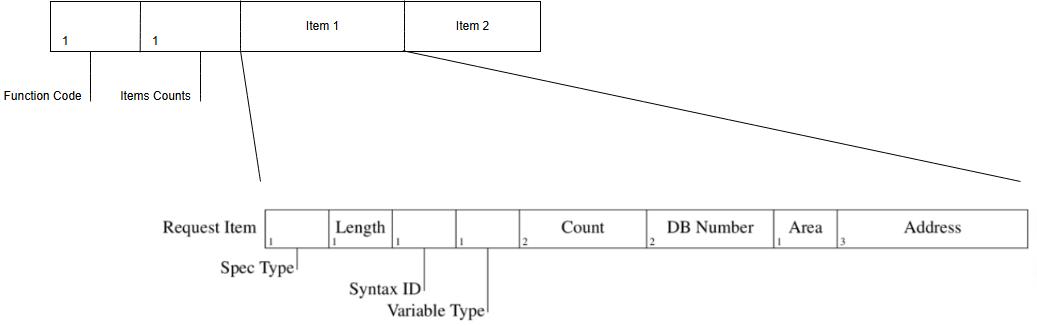
\includegraphics[width=0.85\textwidth]{Figure/AnyTypeStruct.png}
    \caption{Any-type Read Var Param structure}
    \label{fig:stuxnet-anytype-struct}
\end{figure}

\begin{figure}[htbp]
    \centering
    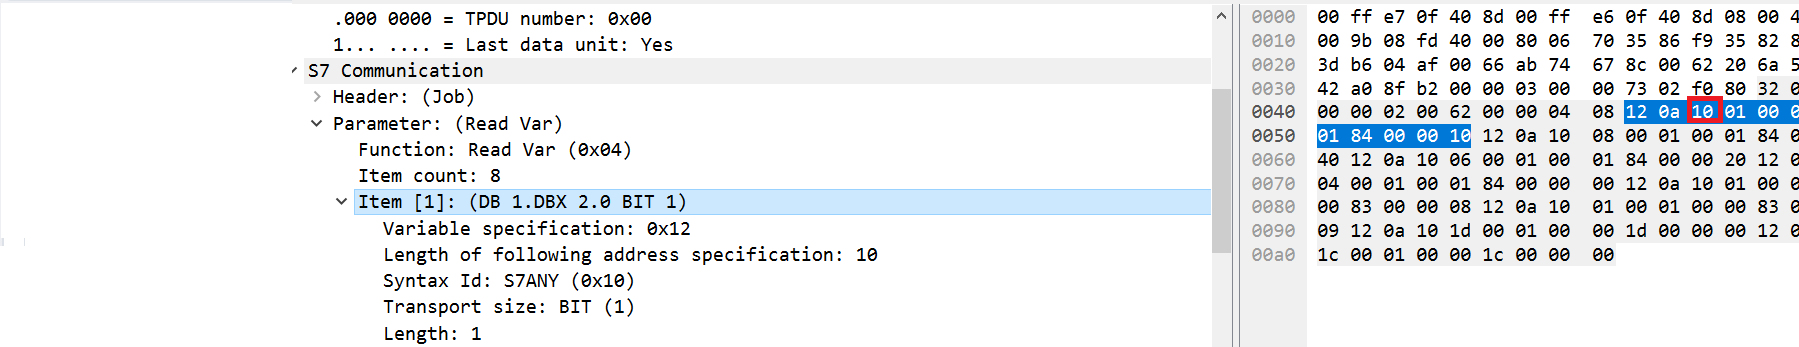
\includegraphics[width=0.9\textwidth]{../attacks/stuxnet_mitm_sim/image-22.png}
    \caption{Any-type addressing in captured traffic}
    \label{fig:stuxnetmitmsimimage22png}
\end{figure}

\begin{figure}[htbp]
    \centering
    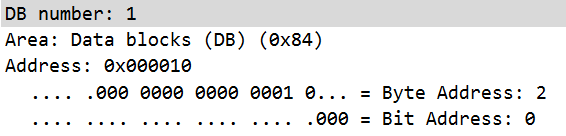
\includegraphics[width=0.9\textwidth]{../attacks/stuxnet_mitm_sim/image-21.png}
    \caption{Any-type request item fields}
    \label{fig:stuxnetmitmsimimage21png}
\end{figure}

\begin{figure}[htbp]
    \centering
    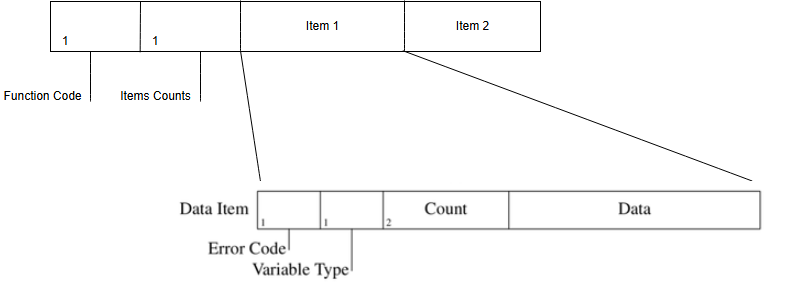
\includegraphics[width=0.85\textwidth]{Figure/ReadVarResponse.png}
    \caption{Read Var response Data item structure}
    \label{fig:stuxnet-readvar-response}
\end{figure}

\begin{figure}[htbp]
    \centering
    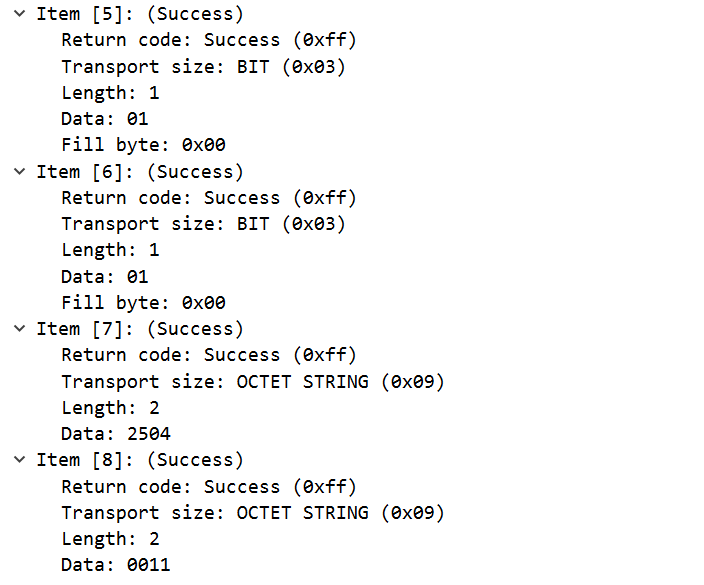
\includegraphics[width=0.9\textwidth]{../attacks/stuxnet_mitm_sim/image-23.png}
    \caption{Read Var response data item}
    \label{fig:stuxnet_mitm_sim-image-23}
\end{figure}

\begin{figure}[htbp]
    \centering
    
\includegraphics[width=0.9\textwidth]{../attacks/stuxnet_mitm_sim/image-24.png}
    \caption{DB-Type request and response items}
    \label{fig:stuxnetmitmsimimage24png}
\end{figure}

Wireshark dissects Param headers reliably but does not always expand Read~Var \emph{Data} payloads to individual tag values. No complete open-source decoder was available for the response layout used here, so the lab reimplemented the field walk described in~\cite{s7_parser_github} as a Python module and checked the output against Wireshark's partial decode (Figure~\ref{fig:stuxnetmitmsimimage16png}). That parser identifies the 29-byte Ack\_Data response that carries both \texttt{iSimSpeed} and \texttt{iSetpoint}; the intercept handler modifies only bytes~27--28 (the setpoint word), recalculates checksums, and reinjects the frame. Editing must keep pace with FUXA polling: a long poll interval delays visible updates even when forgery succeeds (Figure~\ref{fig:stuxnetmitmsimimage27png}).

\begin{figure}[htbp]
    \centering
    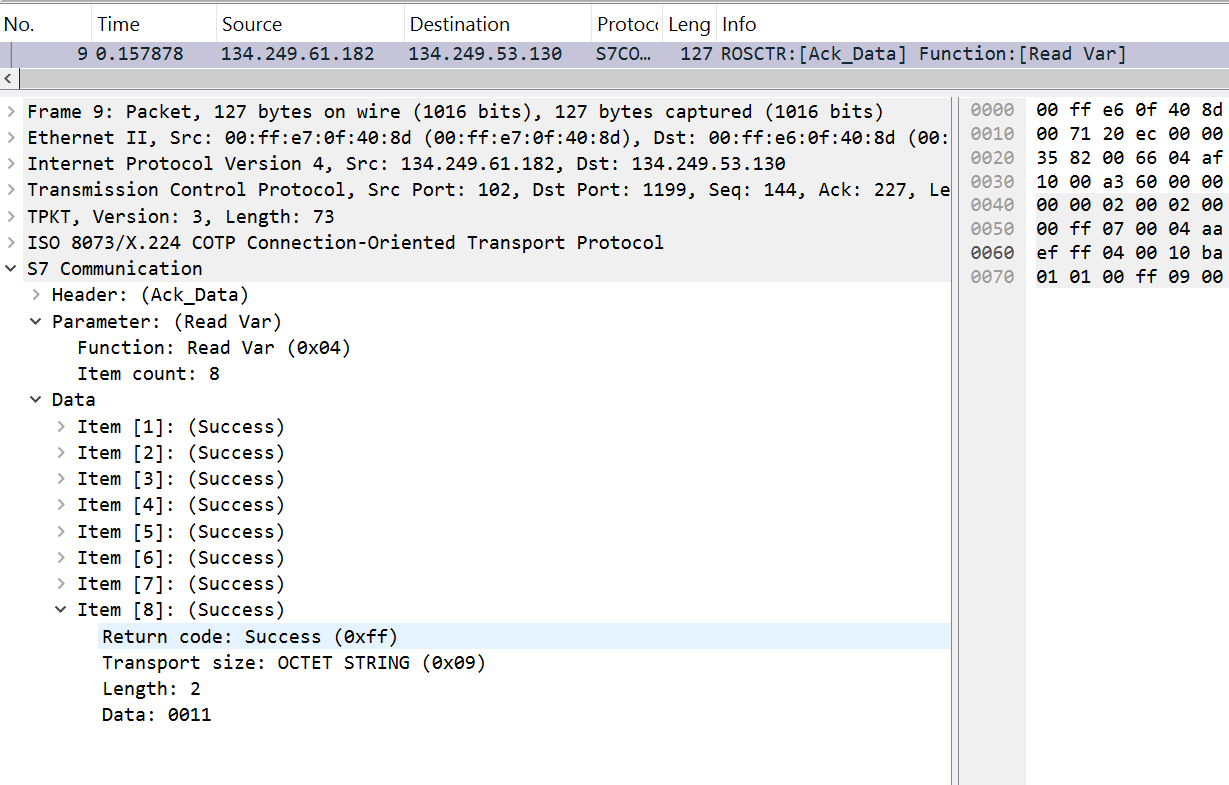
\includegraphics[width=0.9\textwidth]{../attacks/stuxnet_mitm_sim/image-16.png}
    \caption{S7 packet parsed in Wireshark}
    \label{fig:stuxnetmitmsimimage16png}
\end{figure}

\begin{figure}[htbp]
    \centering
    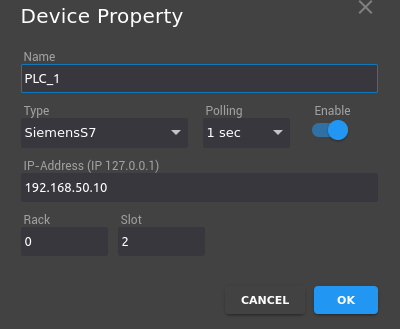
\includegraphics[width=0.9\textwidth]{../attacks/stuxnet_mitm_sim/image-27.png}
    \caption{FUXA HMI polling configuration}
    \label{fig:stuxnetmitmsimimage27png}
\end{figure}
